\documentclass{article}  % Specifies the document class as an article
\usepackage{natbib}      % For citation management and bibliography formatting
\usepackage{listings}    % For including code listings/snippets in the document
\usepackage{xcolor}      % For defining and using custom colors
\usepackage{graphicx}    % For handling images and graphics
\usepackage{fancyhdr}    % For custom headers and footers

% Define custom colors for better contrast
\definecolor{myblue}{rgb}{0.1, 0.2, 0.7}  % Darker blue
\definecolor{mygreen}{rgb}{0.0, 0.5, 0.2}  % Darker green
\definecolor{myred}{rgb}{0.7, 0.1, 0.1}  % Darker red
\definecolor{paleyellow}{rgb}{1.0, 1.0, 0.9}  % Very pale yellow for background

\newcommand{\repoauthor}{\texttt{Thomas Schmelzer}}
\newcommand{\project}{\texttt{Some project}}
\newcommand{\projectnr}{\texttt{10}}
\newcommand{\comment}{\texttt{Confidential}}

% Load git metadata
% Auto-generated by make_header.sh
\usepackage{hyperref}
\newcommand{\commitsha}{\href{https://github.com/tschm/demopaper/commit/782d2bd8ddd430e1e311aeec805921e0dbcf8e89}{\texttt{782d2bd-dirty}}}
\newcommand{\branchname}{\texttt{main}}
\newcommand{\commitdate}{\texttt{2025-07-26}}
\newcommand{\reponame}{\href{https://github.com/tschm/demopaper}{\texttt{tschm/demopaper}}}
\newcommand{\tagname}{\href{https://github.com/tschm/demopaper/releases/tag/v0.5.0-dirty}{\texttt{v0.5.0-dirty}}}


% ===== Header Configuration =====
% Set the page style to fancy (from fancyhdr package)
\pagestyle{fancy}
\fancyhf{}  % Clear all default header and footer fields

% Load fancyvrb for better handling of verbatim text in headers
\usepackage{fancyvrb}
\renewcommand{\headrulewidth}{0.4pt} % Add a line under the header (0.4pt thick)

% Left header: Repository information from header.tex
% This file is dynamically generated by the build system with repo/commit info
\fancyhead[L]{%
  \parbox[t]{0.8\textwidth}{ % Create a paragraph box that takes 80% of text width
    \raggedright\ttfamily\small\textcolor{blue}{Repo: \reponame\\Latest Tag: \tagname, sha: \commitsha} % Left-aligned, monospace, small blue text
  }%
}

% Right header: Current date in blue monospace
\fancyhead[R]{%
  \parbox[t]{0.2\textwidth}{ % Create a paragraph box that takes 20% of text width
    \raggedleft\ttfamily\small\textcolor{blue}{\commitdate} % Right-aligned, monospace, small blue text with current date
  }%
}

\fancyfoot[L]{%
  \parbox[t]{0.8\textwidth}{ % Create a paragraph box that takes 80% of text width
    \raggedright\ttfamily\small\textcolor{blue}{Project: \project, Project Number: \projectnr\\Author: \repoauthor} % Left-aligned, monospace, small blue text
  }%
}

\fancyfoot[R]{%
  \parbox[t]{0.2\textwidth}{ % Create a paragraph box that takes 20% of text width
    \raggedleft\ttfamily\small\textcolor{blue}{\comment} % Right-aligned, monospace, small blue text with current date
  }%
}

% ===== Code Listing Configuration =====
% Configure how code listings will appear in the document
\lstset{
  language=Python,                    % Set the default language for code listings
  basicstyle=\ttfamily\small,         % Use small monospace font for code
  keywordstyle=\color{myblue},        % Darker blue for language keywords
  commentstyle=\color{mygreen},       % Darker green for comments
  stringstyle=\color{myred},          % Darker red for strings
  numbers=left,                       % Show line numbers on the left
  numberstyle=\tiny\color{gray},      % Use tiny gray font for line numbers
  frame=single,                       % Add a single frame around the code
  backgroundcolor=\color{paleyellow}, % Set very pale yellow background for better readability
  breaklines=true,                    % Automatically break long lines
  showstringspaces=false              % Don't show spaces in strings with special symbols
}

% ===== Document Metadata =====
\title{A Brief Overview of the Simple Harmonic Oscillator}  % Document title
\author{Thomas Schmelzer}                                   % Author name
\date{\today}                                               % Current date (automatic)

% ===== Begin Document =====
\begin{document}
\maketitle  % Generate the title based on the metadata above

% Reset page style after \maketitle (which overwrites the fancy style)
\thispagestyle{fancy}  % Apply fancy style to the first page

% ===== Abstract =====
\begin{abstract}
This paper provides a brief overview of the simple harmonic oscillator,
focusing on its mathematical description and physical significance. We discuss
the fundamental equation of motion and its solution, demonstrating why this
system serves as a cornerstone model in physics.
\end{abstract}

% ===== Introduction Section =====
\section{Introduction}
The simple harmonic oscillator is one of the most fundamental models in physics.
Its applications range from the motion of pendulums to the behavior of atoms
in crystal lattices \citep{feynman1963}.  % Citation using natbib package

% ===== Mathematical Description Section =====
\section{Mathematical Description}
The equation of motion for a simple harmonic oscillator is given by:

% Equation 1: The differential equation of motion
\begin{equation}
    \frac{d^2x}{dt^2} + \omega^2x = 0
\end{equation}

where $\omega$ is the angular frequency of oscillation. The general solution
to this equation is:

% Equation 2: The general solution to the equation of motion
\begin{equation}
    x(t) = A\cos(\omega t + \phi)
\end{equation}

where $A$ is the amplitude and $\phi$ is the phase constant
\citep{goldstein2002}.  % Another citation using natbib package

% ===== Code Example Section =====
% Python code example using the listings package with the configuration from above
\begin{lstlisting}
# Python code to calculate sum of squares of first 10 numbers
def sum_of_squares(n):
    return sum(i**2 for i in range(1, n+1))

result = sum_of_squares(10)
print(f"The sum of squares of first 10 numbers is: {result}")
\end{lstlisting}

% ===== Figure Section =====
% [h] attempts to place the figure "here" (can also use [t] for top, [b] for bottom, etc.)
\begin{figure}[h]
\centering                                          % Center the figure horizontally
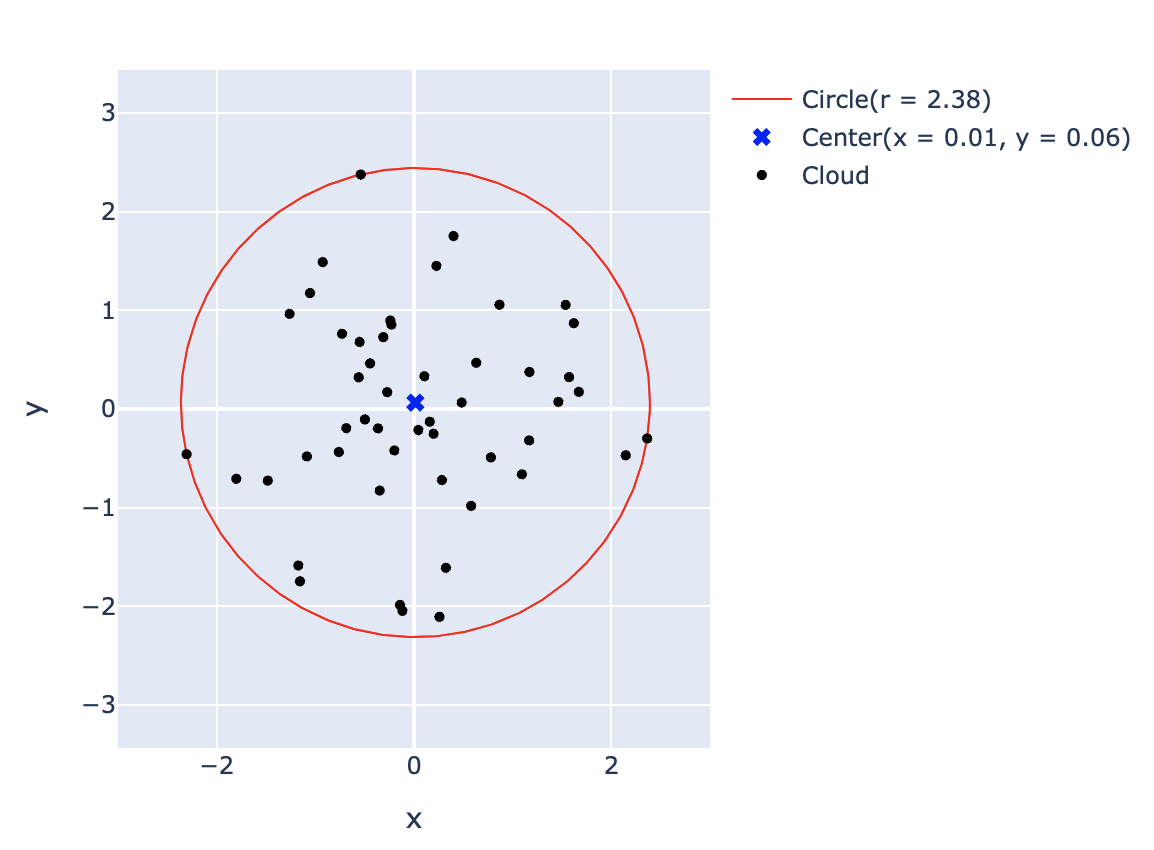
\includegraphics[width=0.8\textwidth]{graph.png}    % Include image scaled to 80% of text width
\caption{This is an example image}                  % Caption text that appears below the figure
\label{fig:example}
\end{figure}

% ===== Bibliography Section =====
% References are stored in the references.bib file in BibTeX format
\bibliography{references}      % Specify the BibTeX file (references.bib)
\bibliographystyle{plainnat}   % Use the plainnat bibliography style (from natbib package)

\end{document}  % End of the document
